\begin{frame}[c]
    \frametitle{用于基于白光 LED 的可见光通信系统的高性能蓝色滤光片}
    \begin{columns}
        \begin{column}{.7\textwidth}
            \begin{itemize}
                \item Wang, S.-W.;  Chen, F.;  Liang, L.;  He, S.;  Wang, Y.;  Chen, X.; Lu, W., A \textcolor{red}{high-performance blue filter} for a white-led-based \textcolor{purple}{visible light communication} system. IEEE wireless communications 2015, 22 (2), 61-67.
                \item \textcolor{blue}{重要性:}基于白光 LED 的可见光通信 (VLC) 系统提供同时照明和高速数据传输,具有高带宽、免许可、低功耗、无电磁干扰、对人体无伤害、高安全性和隐私性等诸多优点。
                \item \textcolor{blue}{创新点:}高目标透射率、尖锐精确的截止边缘、宽阻带。
                \item \textcolor{blue}{瓶颈:}面积大,等效电容高,无法应用于高速运行的情形
                \item \textcolor{blue}{意义:}有效地抑制磷光和环境光成分,提高信噪比、降低误码率,大大提高了 VLC 系统在阳光下或户外使用的能力。
                \item \footnotesize{SNR: Signal Noise Ratio(信噪比),VLC: visible light communication(可见光通信)}
                \item \footnotesize{使用 OptiLayer 软件进行薄膜设计}
            \end{itemize}
        \end{column}
        \begin{column}{.3\textwidth}
            \begin{figure}[H] %H为当前位置,!htb为忽略美学标准,htbp为浮动图形
                \centering %图片居中
                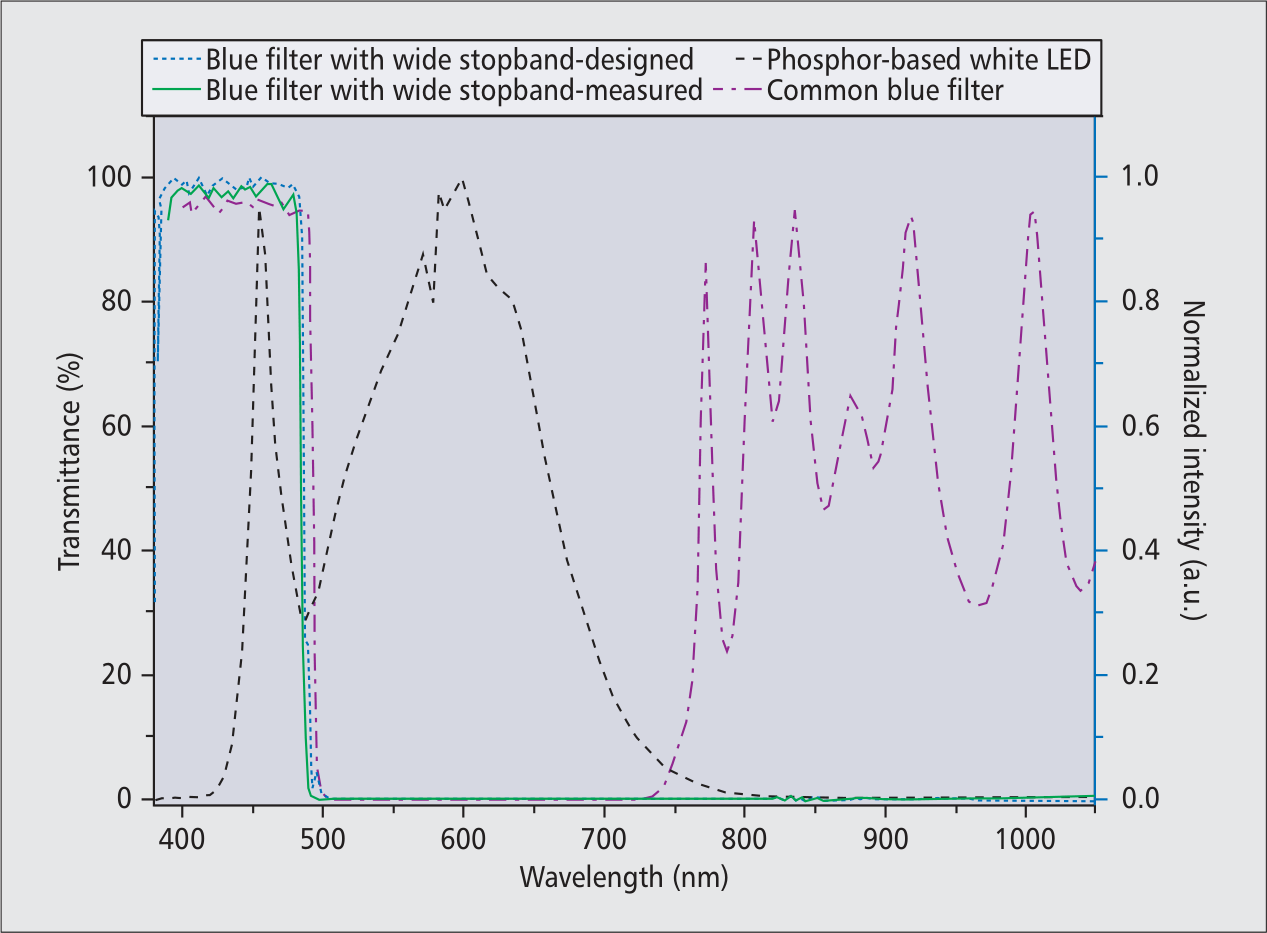
\includegraphics[width=1.1\textwidth]{figures/A high-performance blue filter for a white-led-based visible light communication system_1.png} %插入图片,[]中设置图片大小,{}中是图片文件名
                \caption{透射率} %最终文档中希望显示的图片标题
            \end{figure}
            \begin{figure}[H] %H为当前位置,!htb为忽略美学标准,htbp为浮动图形
                \centering %图片居中
                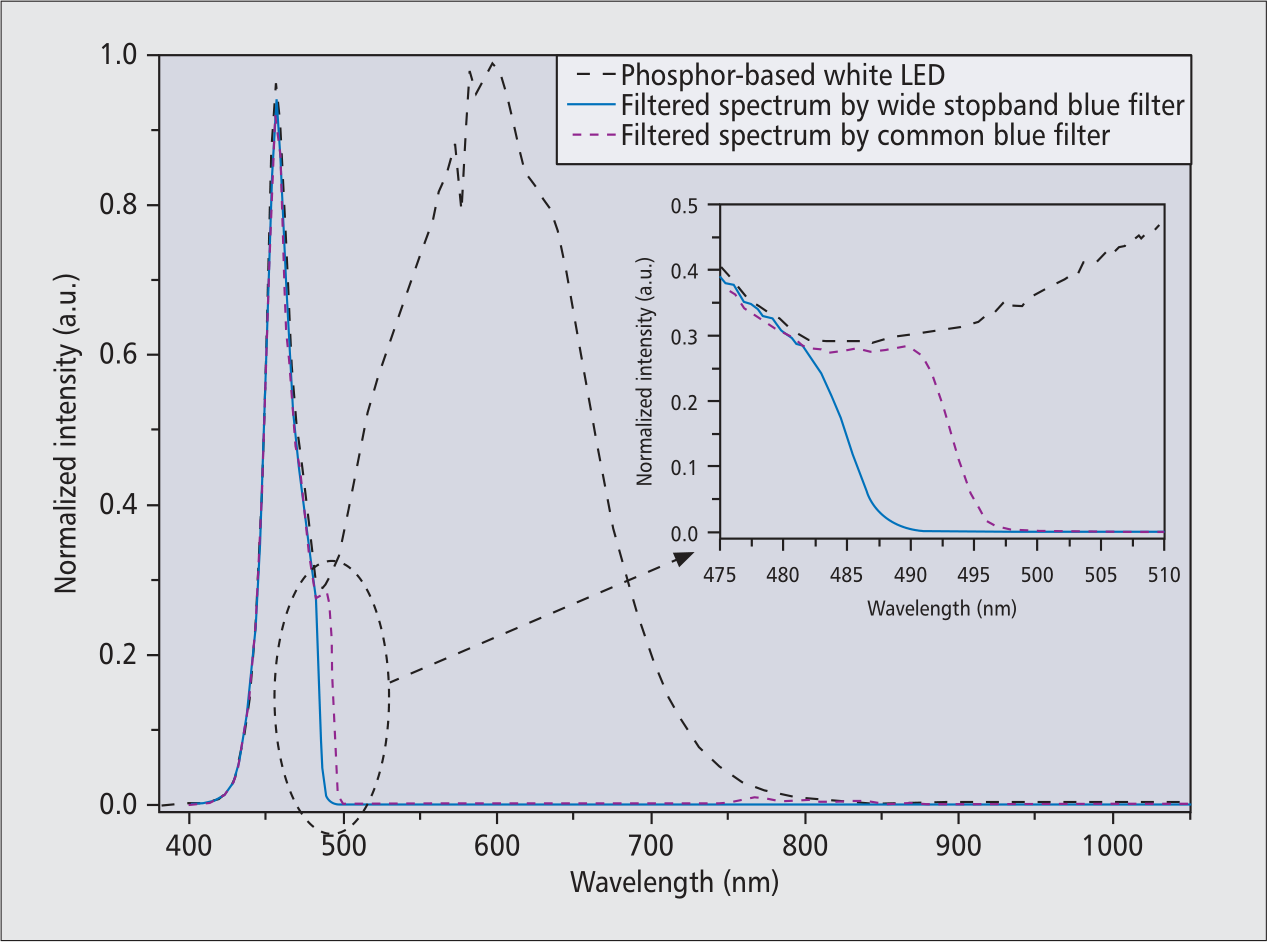
\includegraphics[width=1.1\textwidth]{figures/A high-performance blue filter for a white-led-based visible light communication system_2.png} %插入图片,[]中设置图片大小,{}中是图片文件名
                \caption{光照强度} %最终文档中希望显示的图片标题
            \end{figure}
        \end{column}
    \end{columns}
\end{frame}

\begin{frame}[c]
    \frametitle{用于基于白光 LED 的可见光通信系统的高性能蓝色滤光片}
    一点疑惑:在用文中给出的薄膜结构计算时,只有在忽略介质对光的吸收的情况下才能得到文中的结果,计及介质吸收效应时,薄膜效果极差。
    \begin{columns}
        \begin{column}{.5\textwidth}
            \begin{figure}[H] %H为当前位置,!htb为忽略美学标准,htbp为浮动图形
                \centering %图片居中
                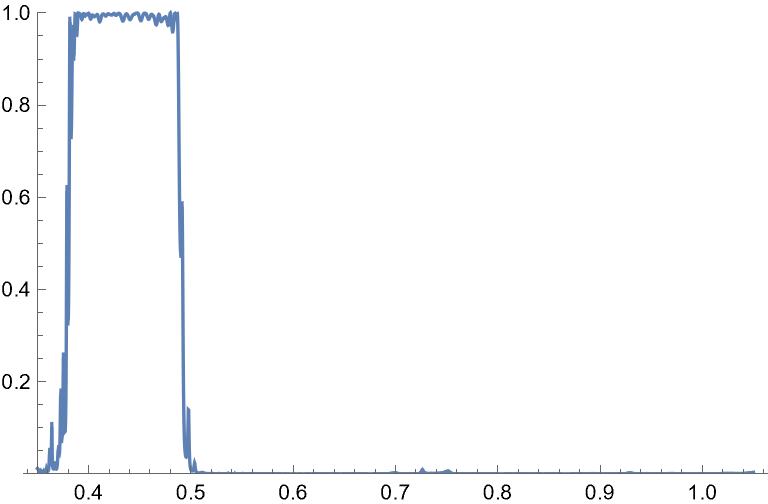
\includegraphics[width=1.\textwidth]{figures/A high-performance blue filter for a white-led-based visible light communication system_3.png} %插入图片,[]中设置图片大小,{}中是图片文件名
                \caption{不考虑介质吸收} %最终文档中希望显示的图片标题
            \end{figure}
        \end{column}
        \begin{column}{.5\textwidth}
            \begin{figure}[H] %H为当前位置,!htb为忽略美学标准,htbp为浮动图形
                \centering %图片居中
                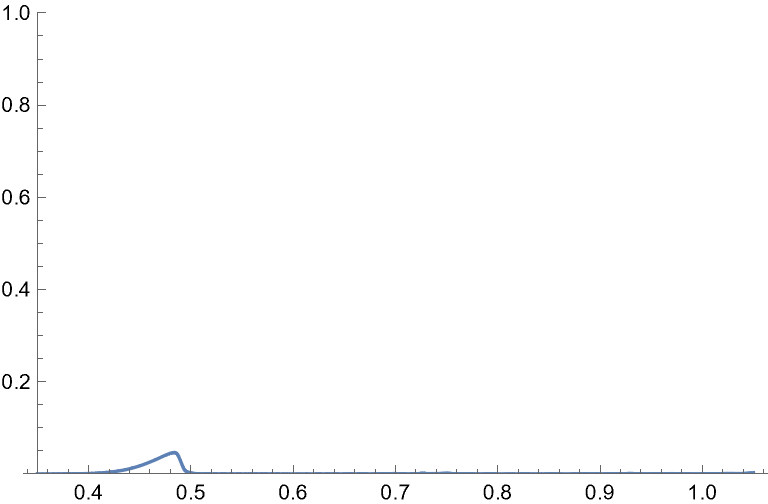
\includegraphics[width=1.\textwidth]{figures/A high-performance blue filter for a white-led-based visible light communication system_4.png} %插入图片,[]中设置图片大小,{}中是图片文件名
                \caption{考虑介质吸收} %最终文档中希望显示的图片标题
            \end{figure}
        \end{column}
    \end{columns}
\end{frame}